\section{Design Approach}
\label{sec:design}

Our system aims to offer the same integrity guarantees as SGX, but also provide
full privacy for the code executing inside a protected container, by hiding the
code's memory access patterns against the attacks described in \S
\ref{sec:sgx_leaks}.

\subsection{The Protected Environment}
\label{sec:protected_environment}


We rely on a protected container that is very similar to an SGX enclave. We
pursue two avenues for designing the container. We will explore a minimal set
of SGX modifications that would prevent against memory access patterns leaking
from enclave execution. We will also explore a clean-slate design that
specifies a minimal set of additions to a RISC architecture resulting in a
protected contained that meets our threat model. Our explorations will contrast
the solutions needed for protecting against both physical and software attacks
against the solutions that only prevent software attacks. We expect that the
latter will have better performance overhead, and want to understand exactly
how the trade-off will work out.

\subsection{The Loader and Verifier}
\label{sec:loader_verifier}

In our system, the infrastructure's kernel or hypervisor is responsible for
creating the protected container and loading our trusted runtime into it. The
runtime loads the untrusted software and private data, and verifies that the
protected container was set up correctly, and that the untrusted software
only interacts with the outside world through the runtime.

We follow the approach of Google Native Client \cite{yee2009native}
\cite{sehr2010adapting}, namely we require that the untrusted software
satisfies some constraints that are easy to verify, and that guarantee that the
software will always interact with the outside world through our trusted
runtime. We provide a compiler that produces code meeting these constraints,
but the compiler is untrusted, and the software provider is free to replace our
compiler with any tool that produces code meeting our constraints. This results
in a small TCB, compared to rewriting the software's machine code on the fly,
and we expect that a technique similar to RockSalt \cite{morrisett2012rocksalt}
can be used to prove the correctness of our verifier. The specific constraints
that we place on software depend on whether protection against physical attacks
is necessary or not, and we cover both cases in the sections below.

SGX has an attestation mechanism that uses a signature of the enclave's initial
contents to set up a secure communication channel between a remote user and
the software running inside the enclave. In our system, the signature only
covers our trusted runtime, reflecting the fact that the software computing on
the private data is not in the TCB.

\subsection{The Memory Manager}
\label{sec:memory_manager}

The x86 address translation (\S \ref{sec:paging}) gives malicious system
software an opportunity to snoop on the enclave software, because of the
information reported by page faults (\S \ref{sec:sgx_leaks}).




\subsection{Software Attacks}

When physical attacks are not taken into account, the main issue of the SGX
design is the handling of CPU faults and interrupts by Asynchronous Enclave
Exits (AEX), which give malicious system software an opportunity to preempt the
enclave software and mount cache timing attacks.

We are investigating servicing faults inside the enclave, instead of performing
an AEX, and asking the local APIC to route interrupts to a different CPU if the
current CPU is executing enclave code. This approach would require the enclave
code to \texttt{EEXIT} in a timely manner, so the system software can schedule
other threads on the CPU. The CPU would prevent against malicious or buggy
enclave code that loops forever by implementing an inter-processor-interrupt
(IPI) that the system software could issue from another CPU core to destroy the
unresponsive enclave and flush the core's caches.

AEX removal would make it impossible for the system software to take advantage
of hyper-threading to snoop on the enclave software by scheduling a malicious
thread on a logical processor in the same core as the logical processor
executing the enclave software. Our runtime would spin loop at start-up, until
the system software schedules enclave threads on all the logical processors
inside the core used to run enclave software.

Our runtime hides the untrusted software's actual running time, which is a
source of information leakage. Instead, the software's metadata specifies a
deadline. If the software does not meet the deadline, it is terminated. If it
does, the runtime spins until the deadline is reached. To implement this, we
prohibit the untrusted software from jumping out of enclave mode (by using
\texttt{EEXIT}) directly, and require that it calls into our runtime instead.
We also require software to call into our runtime periodically, so the runtime
has the opportunity to terminate it. Specifically, the software must call into
our memory manager at the beginning of every basic block. Long basic blocks
must call into our runtime every 100 instructions. This mechanism shall be
tweaked as we gather experience from sample applications.

The requirements mentioned above are enforced by the loader and verifier. We do
not trust the application developer or compiler to produce code that meets
security-sensitive requirements.

We also mention that the deadline-enforcing mechanism in our runtime ensures
that the untrusted software running in an enclave terminates in a timely
manner, so the IPI mechanism described above is not necessary for software
using our runtime, but is required as a part of a sound design for a hardware
protected environment.


\subsection{Physical Attacks}

We prevent against access pattern snooping by devices attached to the
processor's memory bus by obfuscating the memory access patterns. Our trusted
runtime verifies that the software's memory access instructions have been
replaced by calls into our runtime's memory manager.

The memory manager
implements an oblivious RAM (ORAM) protocol \cite{stefanov2013path} to hide the
software's memory access patterns.

The memory manager sets up the L2 cache as a trusted scratchpad. We target the
L2 cache because we trust all the components on the CPU die, and the L2 cache
is the largest on-die cache where the set indexing method is fully documented
(\S \ref{sec:caching}).

The memory manager partitions the sets of the L2 cache into scratchpad sets and
real memory sets. The untrusted software's code and data must only occupy
addresses that map to the real memory sets. The protected environment must also
have a memory area that maps to the scratchpad sets.

\begin{figure}[hbtp]
  \center{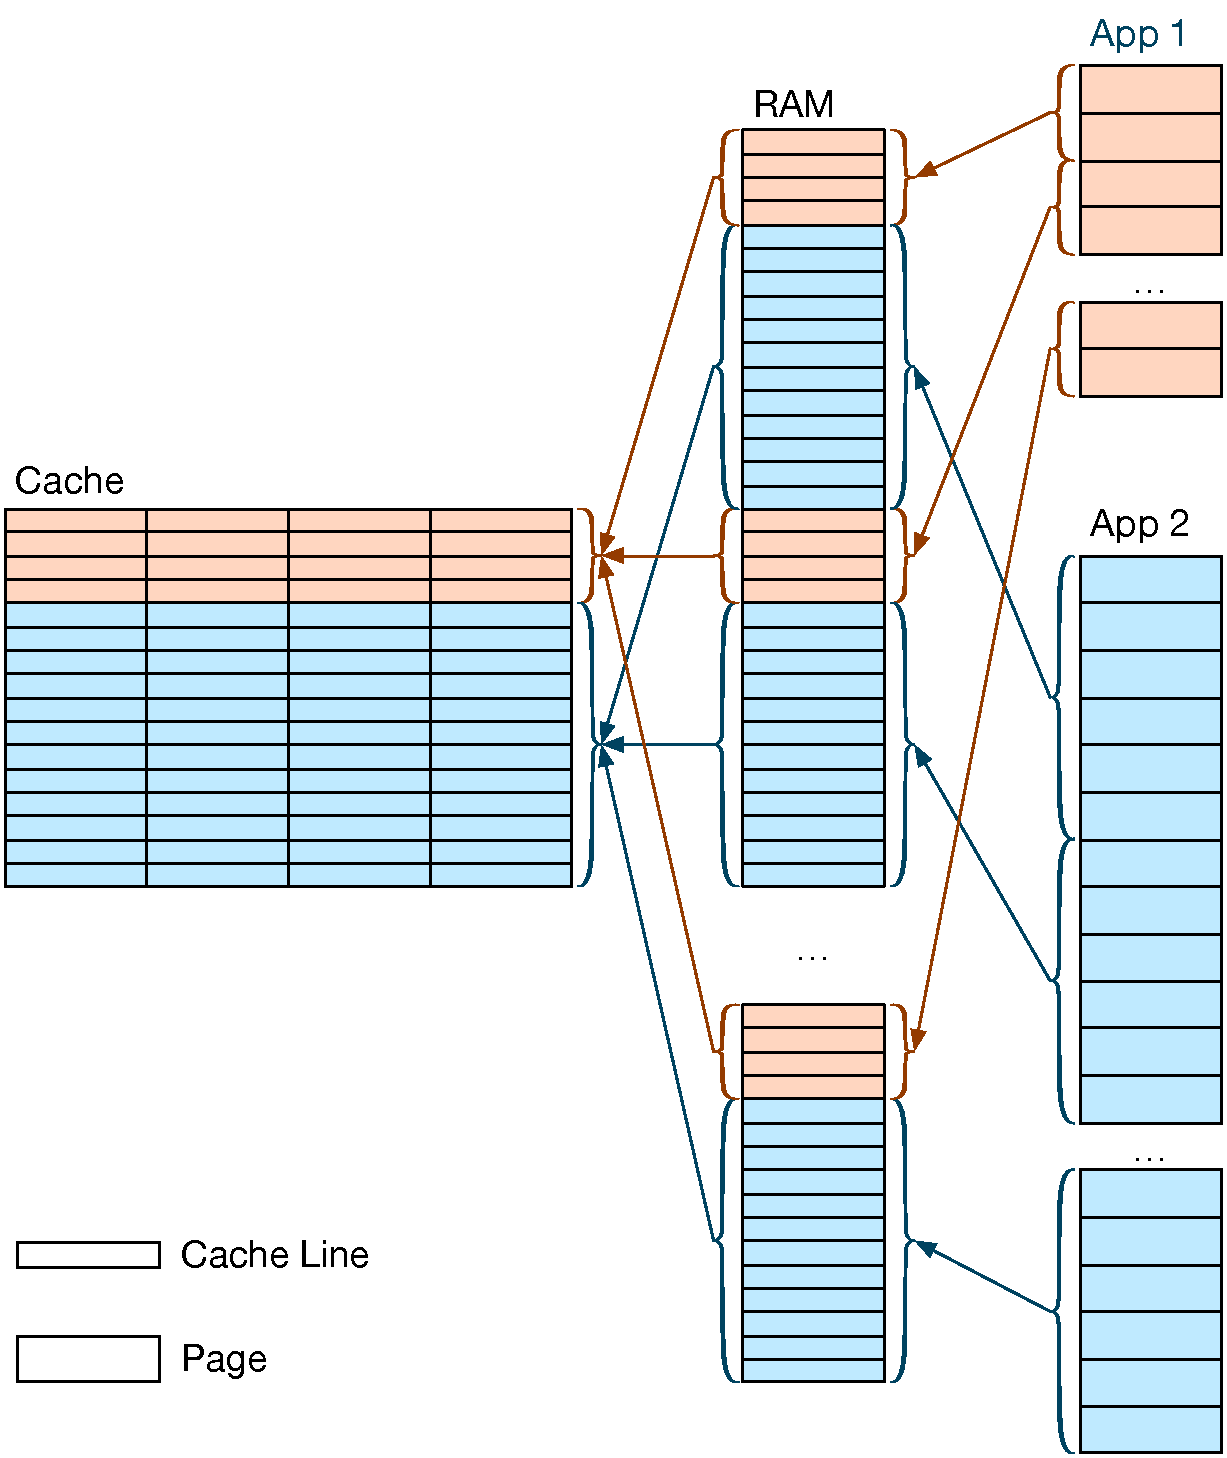
\includegraphics[width=85mm]{figures/cache_partitions.pdf}}
  \caption{
    Cache partitioning between two applications. Each application has some
    cache sets allocated to it, and only uses RAM regions that map to its cache
    sets. When partitioning the L1 cache, applications have to follow this
    constraint themselves. When the L2 cache is partitioned, the OS can map the
    pages in an application's virtual address space to the RAM regions that the
    application can use, so applications are oblivious to the cache
    partitioning.
  }
  \label{fig:cache_partitions}
\end{figure}

The scratchpad is used like a cache for the untrusted software's data. The
memory manager provides functions for reading and writing a memory location.
If the desired location is cached in the scratchpad, it is read or written
immediately. Otherwise, a cache line is evicted from the scratchpad, and
replaced with the line that contains the desired location. If evicted cache
line is dirty, it is written to the software's memory using an ORAM protocol.

To avoid leaking information via memory access timing, the memory manager
runs the ORAM protocol periodically, using the \texttt{RDTSC} instruction as
the clock source. On a read, the memory manager spins in a loop until it can
run the ORAM protocol. Writes are queued up, and the memory manager only spins
in a loop if the queue is full. The untrusted software must also periodically
call into our runtime, so it can run the ORAM protocol at the right time
even if no memory accesses are pending.

System software can also foil the cache partitioning scheme used by our memory
manager, because it controls some of the bits in the physical memory addresses
used to compute the cache set index. We are exploring mechanisms for
constraining the mapping of an enclave page to an EPC page. The extra
constraints would only be checked when an enclave page is created (via
\texttt{EADD}) or loaded into the EPC (via \texttt{ELDB}).

To remain future-proof, the memory manager uses the \texttt{CPUID} instruction
\cite{intel2013manual} to query the CPU's cache layout and aborts when faced
with an implementation that doesn't match our design assumptions.




A simple approach would use one
thread to run enclave code, and spin loop on all the other threads. We are
also considering dedicating a logical processor to the ORAM protocol, and
another logical processor to running the untrusted software.
